\subsubsection{Messung des Stillstandsdrehmomentes}

Im dritten Versuch soll die Konstante $k_e$ bestimmt werden. Diese
beschreibt als Proportionalfaktor den Zusammengang zwischen der
induzierten Spannung $U_i$ und der Winkelgeschwindigkeit $\omega$.

\begin{equation} \label{eq131}
    \begin{split}
        u_i(t)=k_e \cdot \omega (t)
    \end{split}
\end{equation}

Gegeben sind in dieser Aufgabe sind die Messwerte in einer Matrix. Diese
enthält die Spannungswerten von $U_a=U_i$, welche mit einem Multimeter
gemessen worden sind und den Inkrementen pro $\mathrm{ms}$ $Y$, ermittelt
durch einen Inkrementalgeber und einen Mikrocontroller.

Um $k_e$ zu bestimmen wird neben der direkt gegebenen Spannung $U_a$ auch
die Winkelgeschwindigkeit $\omega$ benötigt. Diese ist das Produkt aus
$2\pi$ und der Drehzahl $n$. Während die Winkelgeschwindigkeit angibt wie
schnell sich ein Winkel mit der Zeit um eine Achse ändert, gibt die Drehzahl
die Anzahl der Umdrehungen in einer Zeitspanne an.

\begin{equation} \label{eq132}
    \begin{split}
        k_e = \frac{U_a}{\omega}= \frac{U_a}{2 \pi n}
    \end{split}
\end{equation}

Die gemessen Inkremente pro Zeit müssen daher umgerechnet werden. Diese
wurden mit dem C167 Mikrocontroller mit einer Abtastzeit $T=1\mathrm{ms}$
aufgenommen. Der Inkrementalgeber besitzt 500 Inkremente pro Umdrehung.
Durch eine Vierfachauswertung ergeben sich $P_z=\frac{2000}{2\pi} \mathrm{\frac{INK}{rad}}$.
Dadurch ergibt sich folgender Umrechnungsfaktor $\lambda$.

\begin{equation} \label{eq133}
    \begin{split}
        \lambda = \frac{1000}{P_z} \mathrm{\frac{ms}{s} \frac{rad}{INK}}
    \end{split}
\end{equation}

Über diesen Faktor lässt sich die Drehzahl bestimmen, damit die
Winkelgeschwindigkeit und abschließend auch $k_e$.

\begin{equation} \label{eq133}
    \begin{split}
        n &= \lambda \cdot Y \qquad \text{in} \mathrm{\frac{rad}{s}}\\
        \omega &= 2 \pi \lambda \cdot Y \qquad \text{in} \mathrm{\frac{rad}{s}}\\
        k_e &= \frac{U_a}{2 \pi \lambda \cdot Y}  \qquad \text{in} \mathrm{\frac{Vs}{rad}}
    \end{split}
\end{equation}

Dadurch berechnet sich $ke$ nach über das Reziproke der Steigung der Funktion
multipliziert mit dem Faktor $\lambda$.

\begin{equation} \label{eq134}
    \begin{split}
    k_e = \frac{1}{m \cdot \lambda} \simeq 0.0235 \mathrm{\frac{Vs}{rad}}
    \end{split}
\end{equation}

\begin{figure}[H]
 \centering
 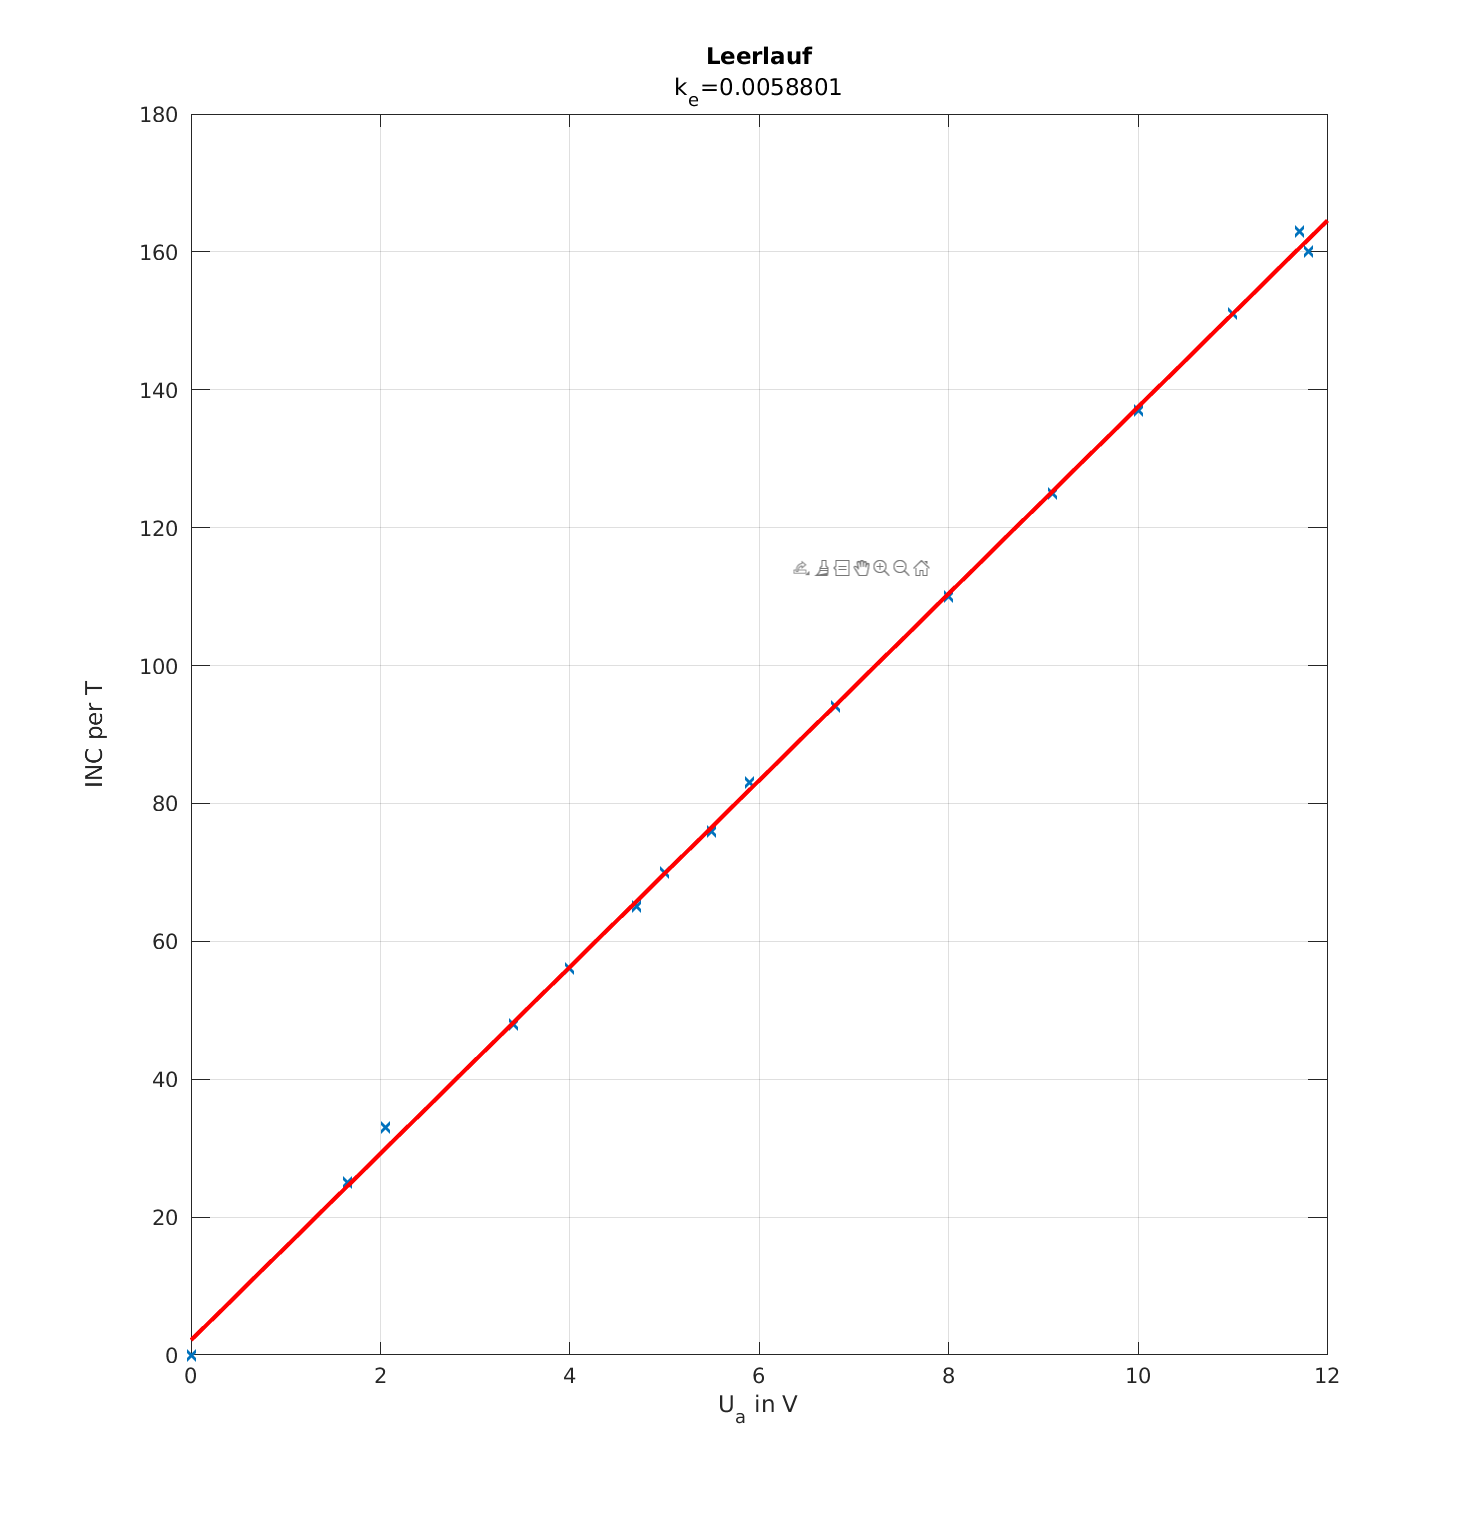
\includegraphics[width=1\textwidth]{as_labor01_3.png}
 \caption{Plot der Aufgabe 3}
 \label{fig:PlotAufgabe3}
\end{figure}